\documentclass{article}

\usepackage{microtype}
\usepackage{graphicx}
\usepackage{subfigure}
\usepackage{booktabs}
\usepackage{amsmath}
\usepackage{amssymb}
\usepackage{multirow}
\usepackage{tikz}
\usetikzlibrary{arrows.meta,positioning}
\usepackage{hyperref}
\usepackage{microtype}
\setlength{\emergencystretch}{2em}

\newcommand{\theHalgorithm}{\arabic{algorithm}}

\usepackage[accepted]{icml2018}

\makeatletter
\renewcommand{\ICML@appearing}{DA-3041 Applied Time Series Analysis course project}
\makeatother

\begin{document}

\twocolumn[
\icmltitle{Volatility Forecasting with the Wavelet Transform: GARCH Model}

% Optional sub-header for course project details
\centerline{\large DA3041 Course Project --- Group 9}
\vskip 0.2in

\begin{icmlauthorlist}
    \icmlauthor{Neeharika Banothu}{dept}
    \icmlauthor{Pratyaksha Jha}{dept}
    \icmlauthor{Pushpendra Singh}{dept}
    \icmlauthor{Somita Agarwal}{dept}
\end{icmlauthorlist}

\icmlaffiliation{dept}{Mehta Family School of Data Science and Artificial Intelligence, IIT Guwahati}
% Adjust affiliation above to match your actual department/institution

% Roll numbers listed cleanly as corresponding emails or equal contribution notes
\icmlcorrespondingauthor{Pushpendra Singh}{github.com/pushpendras0026}
\icmlcorrespondingauthor{Group 9}{240150008, 240150025, 240150026, 240150035}

% You may provide the keywords for the topic:
\icmlkeywords{Volatility Forecasting, Wavelet Transform, GARCH, DA3041}

% \icmlaffiliation{iitg}{Indian Institute of Technology Guwahati, India. DA-3041 Applied Time Series Analysis, Group 9. Roll numbers: 240150008, 240150025, 240150026, 240150035}



\icmlkeywords{volatility forecasting, GARCH, wavelets, DWT, MODWT, time series}

\vskip 0.3in
]
\printAffiliationsAndNotice{}
\begin{abstract}
Forecasting volatility is important for risk management, but daily stock returns are difficult to predict because they are noisy and their variance keeps changing.In the paper \citet{ismail2016} used Haar-type MODWT with ARMA and GARCH(1,1) to forecast volatility in four African stock markets and found that MODWT-GARCH performed better than GARCH(1,1).

We implemented the main methods in R and compared them using rolling one-step-ahead forecasts.We used three African markets (South Africa, Tunisia and Nigeria) and three additional stocks (Infosys, IBM and Google). The data was divided into training (2004–2009), validation (2010–2011) and testing (2012–2014) data. We compared three methods: original returns, paired Haar DWT and Haar MODWT. For each method, we used ARMA to model the mean and GARCH(1,1) to model the variance. We chose the ARMA order using AIC. We kept the target the same for all three methods. It was the squared difference between the next day's return and the average return of the previous 20 days. We also tested the three additional stocks using data from 2015 to 2025.

We also tried Student-t and GED distributions, a structural MODWT order rule, 24 wavelet component models, three equal-weight ensembles and a small MLP with three random seeds. We performed sensitivity analysis using different window lengths, refit frequencies, information criteria and order limits. The Jarque-Bera test rejected normality for all six return series, with kurtosis ranging from 5.24 to 522.53.

Our results showed that MODWT-GARCH had an MSE within 3\% of plain GARCH on all six datasets during 2012–2014. Paired Haar DWT gave lower MSE on Nigeria (9.3\%), Tunisia (7.9\%) and Infosys (3.0\%), although Tunisia had a wide uncertainty interval. Student-t or GED gave the lowest MSE in 23 out of 27 held-out groups, with the largest improvement on Tunisia. Ensembles gave mixed results, while MLP performed worse than GARCH.

From our results, we saw that GARCH(1,1) was already performing well, and it was difficult for the other methods to do better. Wavelet methods gave better results for some datasets, but they did not work better in all cases.
\end{abstract}


%=====================================================================
\section{Introduction}
\label{sec:intro}
Volatility tells us how much a stock price changes over time. Banks and fund managers use volatility forecasts for tasks such as Value-at-Risk, portfolio weights and option pricing. Forecasting volatility is not easy because daily stock returns are noisy, often have extreme values (fat tails), and their variance keeps changing. We can also observe that large movements tend to occur close to each other, which is known as volatility clustering.

GARCH is commonly used to forecast volatility because it considers past shocks and variance. However, it may not capture all the movements that occur at different time scales. To address this, \citet{ismail2016} used Haar-type MODWT along with ARMA and GARCH(1,1) to study four African stock markets: Kenya, Nigeria, South Africa and Tunisia. They reported better forecasting results than the ordinary GARCH model.

We implemented the main methods in R and compared their forecasting performance. The main parts of our work are as follows:

\begin{enumerate}
    \item We implemented three main approaches: GARCH on raw returns, paired Haar DWT-GARCH and Haar MODWT-GARCH.

    \item We compared the methods using rolling one-step-ahead forecasts. In this approach, each forecast uses only the observations available up to that point. We used the validation period to decide the model settings and compared the methods on common test dates.

    \item We used three African markets (South Africa, Tunisia and Nigeria) and three additional stocks (Infosys, IBM and Google). We did not include Kenya because the available NSE-20 data starts only in 2010. The three additional stocks were also tested using a later period, from 2015 to 2025.

    \item We also tried some additional experiments to see if they could improve the results.These included Student-t and GED distributions,wavelet component models,equal-weight ensembles,an MLP and sensitivity analysis.
\end{enumerate}

%=====================================================================
\section{Background and Related Work}
\label{sec:background}

\textbf{ARMA.} An ARMA($p,q$) model is used to describe the behaviour of a time series using its previous values and previous errors (
$\Phi(B)r_t=c+\Theta(B)\varepsilon_t$). ARMA is used mainly to model the mean of the return series. However, it assumes constant error variance and cannot capture volatility clustering properly. In our project, ARMA is used to model the mean before applying GARCH to the residuals. The ARMA order is selected using the Akaike Information Criterion (AIC).

\textbf{GARCH.} \citet{engle1982} introduced ARCH, where the current variance depends on previous squared errors. Later, \citet{bollerslev1986} extended this model by including previous variance, which resulted in the GARCH model. The GARCH(1,1) model can be written as
\begin{equation}
\varepsilon_t=\sqrt{h_t}\,z_t,\qquad h_t=\omega+\alpha\varepsilon_{t-1}^2+\beta h_{t-1},
\label{eq:garch}
\end{equation}
with $\omega>0$, $\alpha,\beta\ge0$ and $\alpha+\beta<1$ for covariance stationarity. GARCH is useful because it captures volatility clustering, where large changes tend to be followed by large changes and small changes tend to be followed by small changes. However, financial returns often contain extreme values and fat tails, which are not always well described by a normal distribution. \citet{hansen2005} showed that it is difficult for other models to consistently outperform GARCH(1,1). To handle fat-tailed returns, \citet{bollerslev1987} used the Student-t distribution, while \citet{nelson1991} introduced the Generalized Error Distribution (GED).

\textbf{Wavelets.} Wavelet transformation is used to analyse a signal at different time scales by separating it into Approximation component(A), which represents smoother movements, and Detail component(D), which represents short-term changes \citet{mallat1989}. In our project, we use two methods: Discrete Wavelet Transform (DWT) and Maximal Overlap Discrete Wavelet Transform (MODWT). DWT uses downsampling, whereas MODWT keeps the same number of coefficients at each level, preserving the time--alignment information of the series. We use the Haar wavelet to find the average and difference between nearby values.

\textbf{Wavelet + GARCH hybrids.} \citet{ismail2016} studied the use of Haar-type MODWT along with ARMA and GARCH(1,1) for forecasting volatility in four African stock markets: Kenya, Nigeria, South Africa and Tunisia. They first transformed the return series using MODWT, selected the ARMA order using AIC and then applied GARCH(1,1) to the transformed series. They compared the results with a normal GARCH(1,1) model and reported improvements in volatility forecasting. They also used statistical tests such as Ljung-Box and ARCH-LM to examine the return series and model residuals. Another study by  \citet{rubio2023} explored wavelet-based ARIMA-GARCH models for forecasting the volatility of Tesla stock.

In our project, we independently implemented three main forecasting approaches: raw returns with GARCH, paired Haar DWT-GARCH and Haar MODWT-GARCH. In the paired Haar DWT approach, neighbouring returns are grouped into pairs and transformed into approximation and detail values. In our MODWT implementation, we use overlapping differences between consecutive returns, calculated as, $w=(r_{2k}-r_{2k-1})/\sqrt2$.We then apply ARMA and GARCH(1,1) to the transformed series and convert the forecasts back to the original return scale. This allows us to compare the wavelet-based approaches with the ordinary GARCH model using the same forecasting target.

We also extended the main experiments by testing 24 wavelet component models on the target series itself. These models use DWT and MODWT with Haar, db4 and db6 wavelet filters at different decomposition levels. The component models were tested using ARMA and GARCH-based approaches to see whether modelling the different components separately could improve forecasting accuracy.

\textbf{Measuring accuracy.} Since actual volatility cannot be directly observed, we use the next squared deviation from the previous 20-day mean as the target. MSE and RMSE are used to compare forecasts. We also use Jarque-Bera, Ljung-Box and ARCH-LM tests to check normality, autocorrelation and remaining ARCH effects.

%=====================================================================
\section{Approach}
\label{sec:approach}

\subsection{Target and rolling protocol}

Let $P_t$ be the closing price and $r_t=\ln P_t-\ln P_{t-1}$ be the daily log return. All three models predict the same target, which is the squared deviation of the next day's return from the previous 20-day average return:
\begin{equation}
y_{t+1}=\bigl(r_{t+1}-\bar r_{t}^{(20)}\bigr)^2,\quad \bar r_t^{(20)}=\tfrac{1}{20}\textstyle\sum_{i=0}^{19}r_{t-i},
\label{eq:target}
\end{equation}
This target is used for all three methods so that their forecasts can be compared fairly. Since the 20-day average is already known at time (t), there is no future information in the target definition.

Each model forecasts one day ahead using the past observations and is re-estimated every 20 trading days. Between refits, the model parameters remain fixed, but the forecasts use the latest available observations. We also checked for data leakage to make sure future values do not affect earlier forecasts.

If a model gives the next return's conditional mean  $\mu_{t+1}$ and variance $h_{t+1}$  its forecast of the target is
\begin{equation}
\hat y_{t+1}=h_{t+1}+\bigl(\mu_{t+1}-\bar r_t^{(20)}\bigr)^2 ,
\label{eq:restore}
\end{equation}
because $E[(r-m)^2]=\mathrm{Var}(r)+(E r-m)^2$.

This follows from the expected squared deviation being equal to the variance plus the squared difference between the mean and the reference value.

\subsection{Mean and variance models}

For each input series, we select the ARMA($p,q$) order with $p,q\le3$ using AIC $=-2\ell+2k$ on the latest 1,024 observations in the training window. AIC helps us choose a model that fits the data without using too many parameters. The ARMA model is estimated using Gaussian maximum likelihood, and GARCH(1,1) is then fitted to its residuals. We use this two-step approach because it is simpler to implement and compare. For the raw returns, the selected ARMA orders are (3,1) for South Africa, (2,0) for Tunisia, (0,3) for Nigeria, (0,3) for Infosys, (2,2) for IBM and (3,3) for Google.The estimated GARCH persistence $\alpha+\beta$  ranges from 0.93 to 0.997 across the six series, showing that volatility shocks have a lasting effect.

\subsection{The three pipelines}

\begin{figure}[H]
\centering
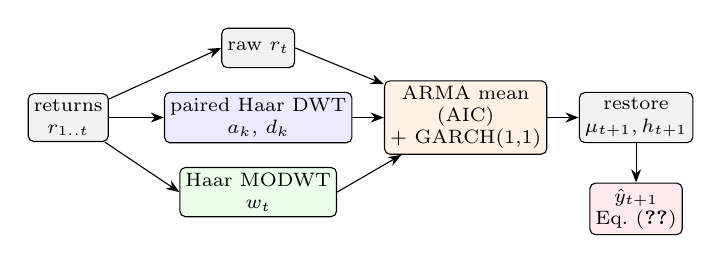
\begin{tikzpicture}[>=Stealth, font=\scriptsize, node distance=3mm and 2mm,
 box/.style={draw, rounded corners=2pt, align=center, minimum height=5mm, inner sep=2pt}]
\node[box, fill=black!5] (r) {returns\\$r_{1..t}$};
\node[box, right=7mm of r, fill=blue!8] (dwt) {paired Haar DWT\\$a_k,\,d_k$};
\node[box, above=of dwt, fill=gray!10] (raw) {raw $r_t$};
\node[box, below=of dwt, fill=green!8] (mod) {Haar MODWT\\$w_t$};
\node[box, right=4mm of dwt, fill=orange!10] (am) {ARMA mean\\(AIC)\\+ GARCH(1,1)};
\node[box, right=4mm of am, fill=black!5] (rs) {restore\\$\mu_{t+1},h_{t+1}$};
\node[box, below=5mm of rs, fill=red!8] (y) {$\hat y_{t+1}$\\Eq.~(\ref{eq:restore})};
\draw[->] (r) -- (raw.west);
\draw[->] (r) -- (dwt);
\draw[->] (r) -- (mod.west);
\draw[->] (raw.east) -- (am);
\draw[->] (dwt) -- (am);
\draw[->] (mod.east) -- (am);
\draw[->] (am) -- (rs);
\draw[->] (rs) -- (y);
\end{tikzpicture}
\caption{The three core pipelines. Each input branch gets its own ARMA--GARCH, and the forecast is mapped back to the common target.}
\label{fig:pipe}
\end{figure}

Figure~\ref{fig:pipe} shows the three approaches used in our project. The raw GARCH model uses the original returns, while the other two first apply Haar wavelet transformations. We implemented both paired Haar DWT and overlapping Haar MODWT to compare their performance.

\textbf{Raw GARCH.} This is our basic model. We directly apply ARMA to the original returns to estimate the mean and then GARCH(1,1) to estimate the variance.

\textbf{MODWT-GARCH.} Here, we first calculate the Haar detailvalues using overlapping differences between consecutive returns:$w_t=(r_t-r_{t-1})/2$. We then model this series using ARMA-GARCH. Since $r_{t+1}=r_t+2w_{t+1}$ and $r_t$is already known, the forecast mean and variance of theoriginal return are obtained as $\hat{\mu}_{r,t+1}=r_t+2\hat{\mu}_{w,t+1}$ and
$\hat{h}_{r,t+1}=4\hat{h}_{w,t+1}$.


\textbf{Paired DWT-GARCH.} In this approach, we group consecutive returns into non-overlapping pairs $(u_k,v_k)$ and calculate their Haar approximation and detail values: $a_k=(u_k+v_k)/\sqrt{2}$ and
$d_k=(v_k-u_k)/\sqrt{2}$. We fit separate ARMA-GARCH models to both series to obtain their forecast means and variances $(\mu_a,h_a)$ and $(\mu_d,h_d)$. The important part is that the first return $r_t$ of the next pair is already known when forecasting $r_{t+1}$. So, we use this information to calculate
the conditional forecast. Assuming the approximation and detail are jointly normal and uncorrelated, we get $s=a-d=\sqrt{2}r_t$, and the conditional detail mean is
\begin{align}
E[d\mid s]
&=\mu_d-\frac{h_d}{h_a+h_d}
\left(s-(\mu_a-\mu_d)\right).
\end{align}
Using this, the forecast mean and variance of the next return are calculated as
\begin{align}
\hat{\mu}_r &= r_t+\sqrt{2}E[d\mid s],\\
\hat{h}_r &= \frac{2h_ah_d}{h_a+h_d}.
\end{align}



\subsection{Evaluation}
We use MSE as the main measure and RMSE
to compare the forecasts on the test data. We also calculate the percentage improvement over raw GARCH using $100(1-\mathrm{MSE}_{\text{model}}/\mathrm{MSE}_{\text{raw}})$.A positive value means that the model performs better than raw GARCH. Some model fits fail because the optimiser does
not converge, so we compare models only on dates where all
of them have valid forecasts. This can lead to different
numbers of test observations in different result tables.


%=====================================================================
\section{Our Extensions}
\label{sec:ext}

The paper only assumes Gaussian distribution on GARCH on African indices. We added the following extensions. The paper chose 2010-2011 validation period and settings were kept the same for test set.

\textbf{E1: Student-t distribution and GED.} Our tests (Table~\ref{tab:data}) show that all six datasets reject normality test, so using a Gaussian $z_t$ in Eq.~(\ref{eq:garch}) is not accurate. We again fit each of the three pipelines using a standardized Student-t (shape $\nu$) distribution and with a GED (shape $\kappa$), keeping the same ARMA mean, window and procedure. We calculated likelihoods for both process using \texttt{optim}.

\textbf{E2: structural MODWT order.} Multiplying a raw ARMA($p,q$) by the Haar filter $(1-B)/2$ adds one MA lag, so the MODWT detail should follow ARMA($p,q+1$). We tried this rule (with Gaussian and Student-t) as an alternative to choosing the MODWT order by AIC. The validation period picks between them per series.

\textbf{E3: wavelet component models of the target.} Instead of transforming returns, we also decompose the target $y$ itself into $A_J$ and $D_J,\dots,D_1$ , forecast each part and sum them.The approximation is put into ARMA and the detail part is put into GARCH.

\textbf{E4: Ensemble learning.}  We built three ensembles, without fitting any weights on the test: \emph{base} (the six raw/DWT/MODWT ARMA and GARCH forecasts), \emph{combined} (base plus the direct-target ARMA and four selected component models) and \emph{MODWT} (two MODWT return models and two MODWT component models).

\textbf{E5: Neural network.} We also implement a hidden-layer MLP  with 7 inputs (the last five targets and the past 5-day and 20-day mean), 3 or 5 sigmoid units, weight decay 0.001 or 0.01, and a linear output.We test over three seeds (101, 202, 303) and use validation MSE to determine size and decay, and we report all three seeds on the test.

\textbf{E6: Change in settings.} For the three  pipelines we change one setting at a time: window 768 or 1,536 (instead of 1,024), refit every 40 or 60 days (instead of 20), use BIC instead of AIC.

\textbf{E7: More markets and a later period.} Besides three of the paper's African indices we add Infosys (India), IBM and Google (USA), and for the stocks we also run the models on 2015--2025.

%=====================================================================
\section{Experiments}
\label{sec:exp}

\subsection{Data and setup}

The daily closing prices were obtained from the following public data sources : FTSE/JSE All Share (South Africa), TUNINDEX (Tunisia) and the NGX All Share Index (Nigeria), and Yahoo Finance adjusted closes for Infosys, IBM and Google. We kept all trading dates and did not interpolate or fill the data. We kept a record of the inconsistencies in the data, for example Tunisia has two returns of $-0.27$ and $+0.27$ on 15--16 Sep 2004. Training was done on data from 2004 to 2009 (about 1,350--1,510 returns), validation on 2010--2011 (about 500 returns) and test 2012--2014 (about 750 returns). The stocks have about 2,700 more days in 2015--2025.

The code is written in R and \texttt{nnet} is used for MLP. Jobs run in parallel on 16 cores. The code and supplementary materials are available on \href{https://github.com/pushpendras0026/Volatility-forecasting-with-the-wavelet-transform}{Github}.

\begin{table}[t]
\caption{Full-sample daily log returns (2004 to 2014 for indices, to 2025 for stocks). Kurt is raw kurtosis (normal $=3$). JB: Jarque--Bera $p$. ADF and KPSS are statistics; all ADF $p<10^{-4}$.}
\label{tab:data}
\centering\small
\setlength{\tabcolsep}{3.5pt}
\begin{tabular}{lrrrrrr}
\toprule
Series & $n$ & Skew & Kurt & JB $p$ & ADF & KPSS \\
\midrule
S.\ Africa & 2750 & $-0.18$ & 6.90 & $<10^{-4}$ & $-25.9$ & 0.147 \\
Tunisia & 2720 & $-0.38$ & 522.53 & $<10^{-4}$ & $-64.3$ & 0.463 \\
Nigeria & 2722 & 0.00 & 5.24 & $<10^{-4}$ & $-25.4$ & 0.180 \\
Infosys & 5444 & $-0.58$ & 14.89 & $<10^{-4}$ & $-45.2$ & 0.055 \\
IBM & 5534 & $-0.34$ & 12.36 & $<10^{-4}$ & $-22.9$ & 0.124 \\
Google & 5376 & 0.32 & 10.67 & $<10^{-4}$ & $-28.4$ & 0.108 \\
\bottomrule
\end{tabular}
\end{table}

\textbf{Data checks.} Following \citet{ismail2016} and \citet{rubio2023} we first tested the returns (Table~\ref{tab:data}). Every series has kurtosis above 3 and the Jarque--Bera test rejects normality with $p<10^{-4}$. Tunisia's kurtosis of 522 is mostly from the two September 2004 days. The ADF test rejects a unit root for all series and KPSS does not reject stationarity at 5\% (Tunisia is borderline with 0.463), so returns can be modelled without differencing. After fitting, the ARCH-LM test on the plain ARMA residuals was very significant ($p\approx10^{-45}$ for South Africa) while on the standardized GARCH residuals it was not significant, so GARCH effectively captures the clustering.

\subsection{Core result: raw vs.\ DWT vs.\ MODWT}

\begin{table}[t]
\caption{Test RMSE $\times10^4$, 2012--2014, Gaussian GARCH. Matched dates on which all three models have a forecast. Bold is the lowest in each row. Gain is MSE reduction vs.\ raw (\%).}
\label{tab:core}
\centering\small
\setlength{\tabcolsep}{3pt}
\begin{tabular}{lrrrrrr}
\toprule
Series & $n$ & Raw & DWT & MODWT & \multicolumn{2}{c}{Gain \%} \\
 & & & & & DWT & MODWT\\
\midrule
S.\ Africa & 749 & 1.3426 & 1.3448 & \textbf{1.3394} & $-0.3$ & $+0.5$\\
Tunisia & 745 & 0.7076 & \textbf{0.6790} & 0.7061 & $+7.9$ & $+0.4$\\
Nigeria & 745 & 1.8920 & \textbf{1.8015} & 1.9173 & $+9.3$ & $-2.7$\\
Infosys & 736 & 25.3177 & \textbf{24.9339} & 25.2165 & $+3.0$ & $+0.8$\\
IBM & 751 & \textbf{4.1300} & 4.1585 & 4.1305 & $-1.4$ & $0.0$\\
Google & 752 & 7.7822 & 7.7857 & \textbf{7.7781} & $-0.1$ & $+0.1$\\
\bottomrule
\end{tabular}
\end{table}

Table~\ref{tab:core} shows that differences in RMSE are very small. MODWT-GARCH is within about 3\% MSE of raw GARCH on every series; it is better on four datasets and worse on Nigeria. Hence, with Haar, the MODWT detail part is a fixed linear filter of the returns, and an ARMA on a filtered series can give same results as what an ARMA on the returns can already do. The paired DWT performs better: it is the best model on Tunisia, Nigeria and Infosys, with 7.9\%, 9.3\% and 3.0\% lower MSE, and close to baseline on the other three stocks. The gain intervals are positive for Nigeria ($0.5$ to $17.6\%$) and Infosys ($1.4$ to $14.9\%$) but very wide for Tunisia ($-20.7$ to $14.9\%$), so the Tunisia gain is not reliable. A possible reason is that the DWT models two coefficient series with their own GARCH, so on the less volatile African markets it can react to short shocks differently. However, on IBM and Google, with high volatility,raw GARCH performs the best

The baseline models used for reference give mixed results(each on its own available dates). It ($\hat y_{t+1}=y_t$) is worse than raw GARCH on all six series, for example RMSE 1.951 vs.\ 1.343 on South Africa. A plain ARMA with constant variance is worse on four series (1.705 on South Africa) but slightly better on Tunisia and Infosys, and the 20-day trailing mean of $y$ even beats GARCH on Tunisia (0.663 vs.\ 0.708). The Tunisia test target is very small and rapidly fluctuating, so a smooth average does well there. Overall the GARCH part does most of the work, and the wavelet step improves it by a small amount at best.Figure~\ref{fig:tun} shows that the forecasts follow the big spikes of the target only after they happen, which is what we expect from any one-step GARCH-type model.

\begin{figure*}[t]
\centering
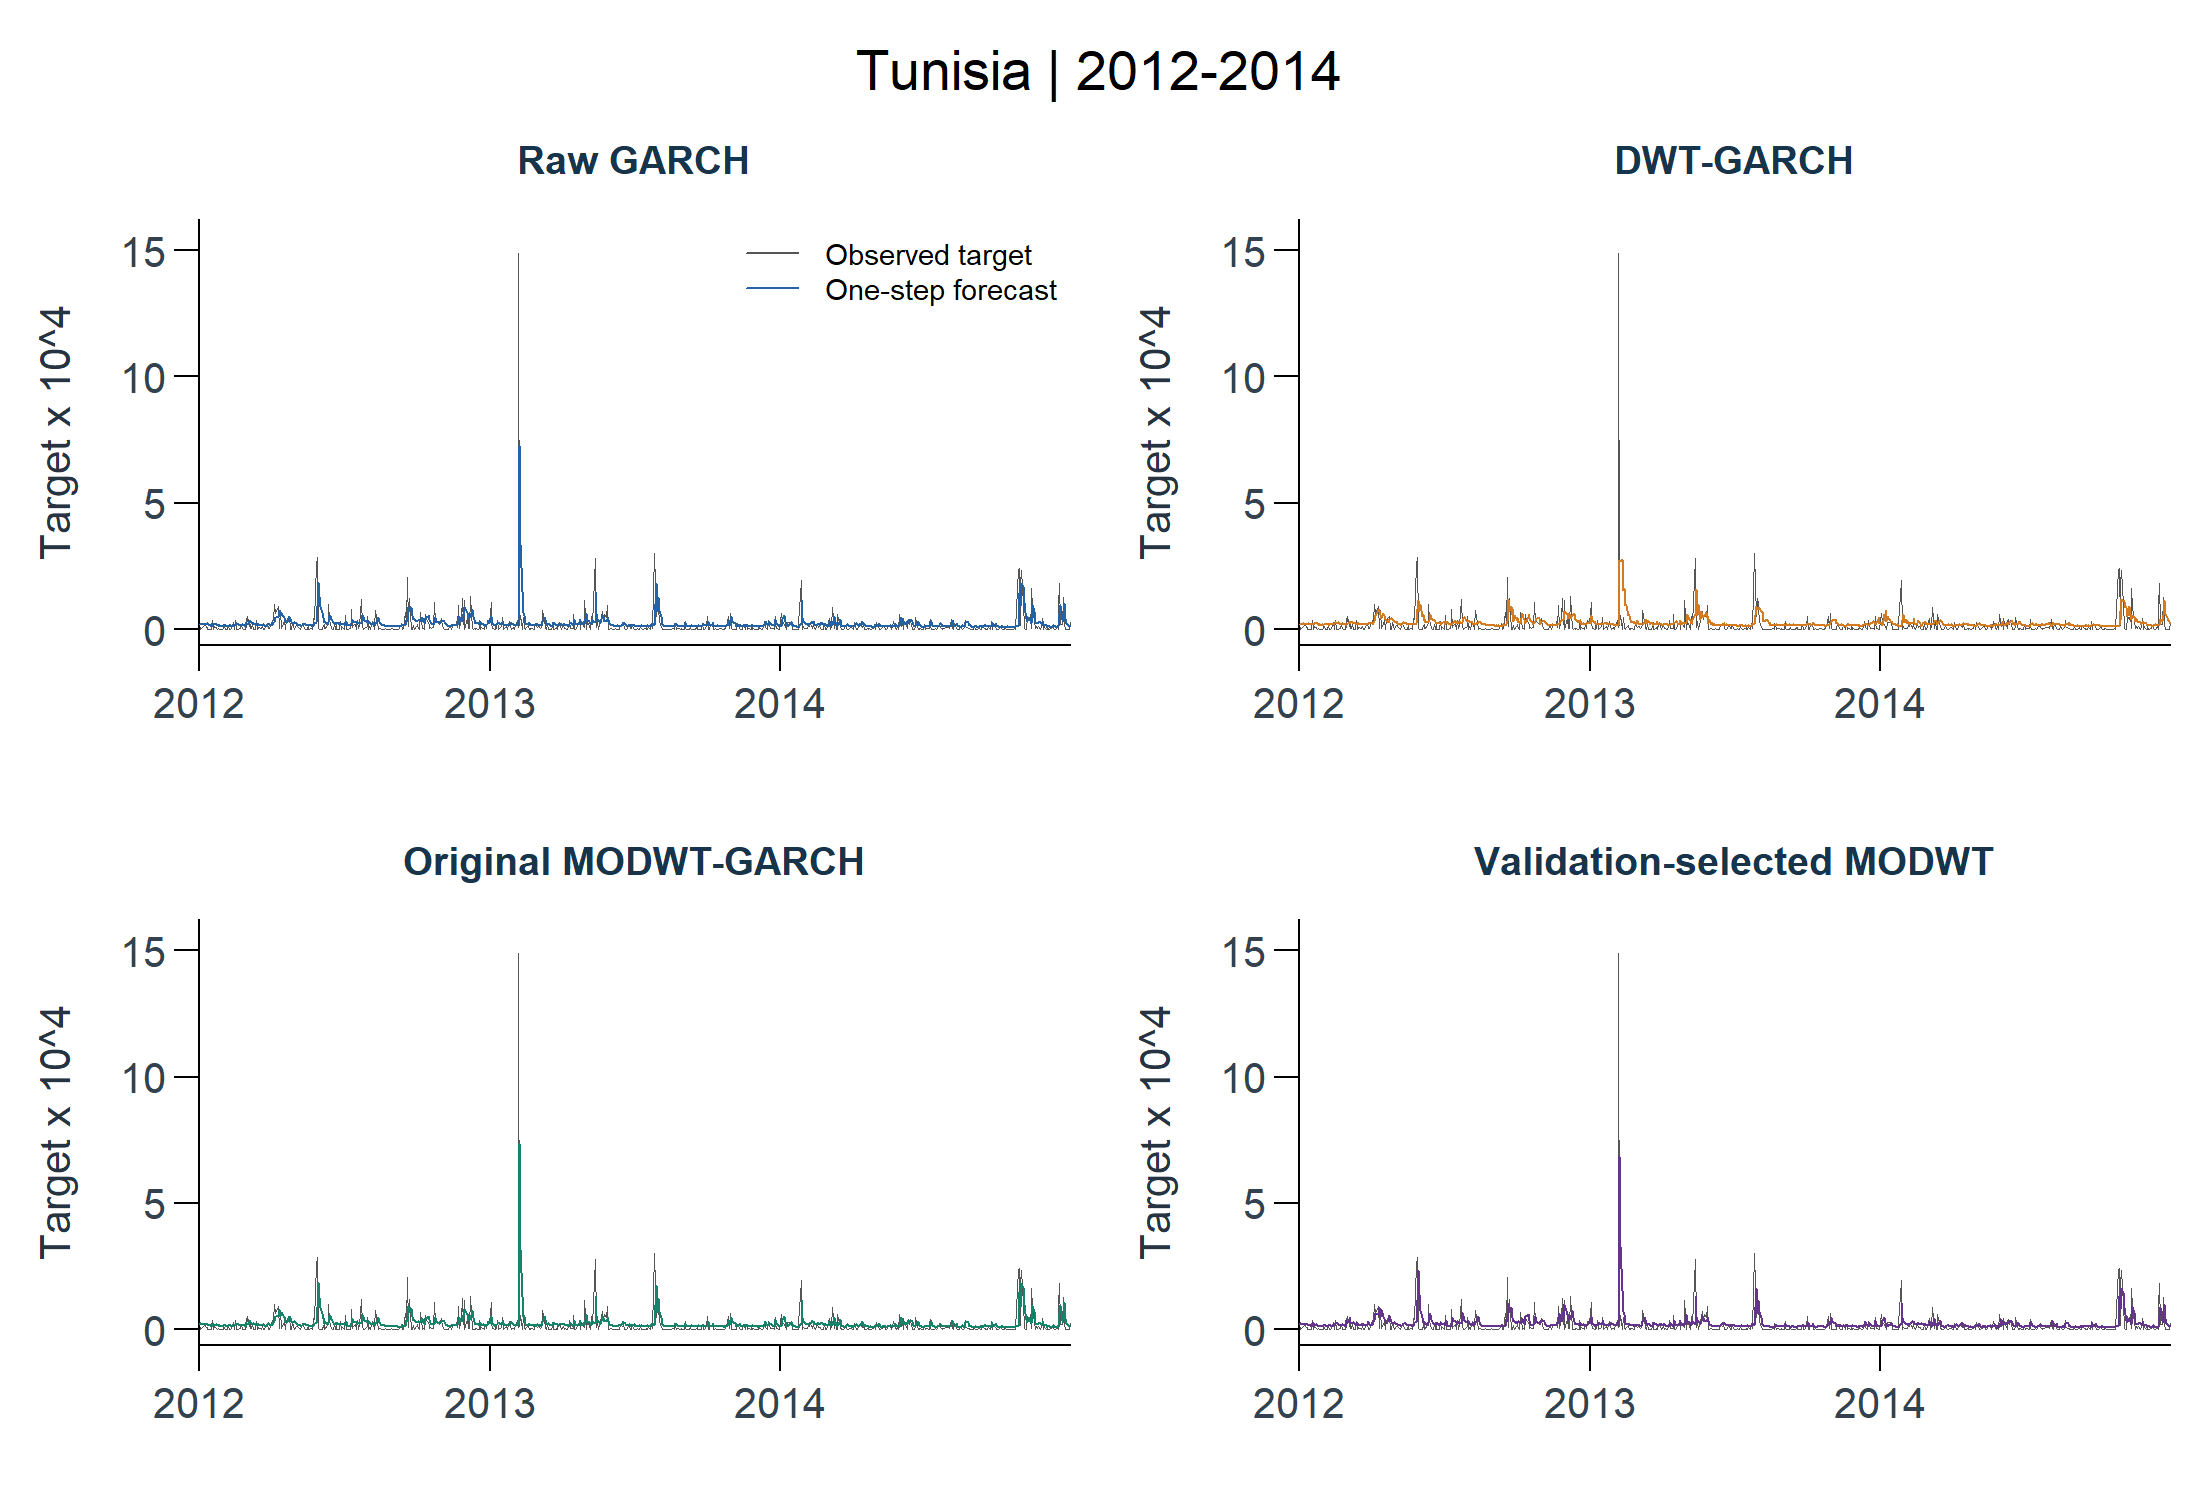
\includegraphics[width=0.78\textwidth]{figures/tunisia_test_core.png}
\caption{Tunisia, 2012--2014 test: observed target (grey) and one-step forecasts. The ``validation-selected MODWT'' panel is the Student-t MODWT model chosen by E2/E1 on validation. All models react after the shock in early 2013, not before.}
\label{fig:tun}
\end{figure*}

\subsection{Fat-tailed innovations (E1)}

\begin{table}[t]
\caption{Raw GARCH test RMSE $\times10^4$ (2012--2014) under three innovation distributions. Last row indicates the number of the 27 held-out groups (series $\times$ pipeline $\times$ period, incl.\ 2015--2025) where each distribution has the lowest MSE.}
\label{tab:dist}
\centering\small
\begin{tabular}{lrrr}
\toprule
Series & Gaussian & Student-t & GED\\
\midrule
S.\ Africa & 1.3426 & \textbf{1.3421} & 1.3423\\
Tunisia & 0.7076 & \textbf{0.6998} & 0.7016\\
Nigeria & 1.8920 & \textbf{1.8853} & 1.8901\\
Infosys & 25.3009 & \textbf{24.9601} & 25.1028\\
IBM & 4.1300 & 4.1352 & \textbf{4.1296}\\
Google & 7.7822 & 7.7715 & \textbf{7.7649}\\
\midrule
Lowest MSE & 4 & 13 & 10\\
\bottomrule
\end{tabular}
\end{table}

Table~\ref{tab:dist} shows that a fat-tailed distribution improves the results in all of our datasets. Over the 27 held-out groups (6 series $\times$ 3 pipelines in 2012--2014 and 3 stocks $\times$ 3 pipelines in 2015--2025), Student-t has the lowest MSE in 13 and GED in 10, while Gaussian has the lowest in 4 cases. On MAE GED is best in 18 groups. The gains are small, the median MSE change of Student-t vs.\ Gaussian is about $-0.3\%$ in 2012--2014 and $-1.2\%$ in 2015--2025, but they mostly go in the right direction. The biggest gain is on Tunisia, which has the fattest tails: DWT-GARCH goes from 0.6790 to 0.6564 with Student-t (6.6\% lower MSE). The reason is that with fat tails, a Gaussian likelihood over-reacts to one huge return, and the t or GED likelihood down-weights it, giving more stable $\alpha$ and $\beta$.

\subsection{Component models, ensembles and MLP (E3--E5)}

\begin{figure}[t]
\centering
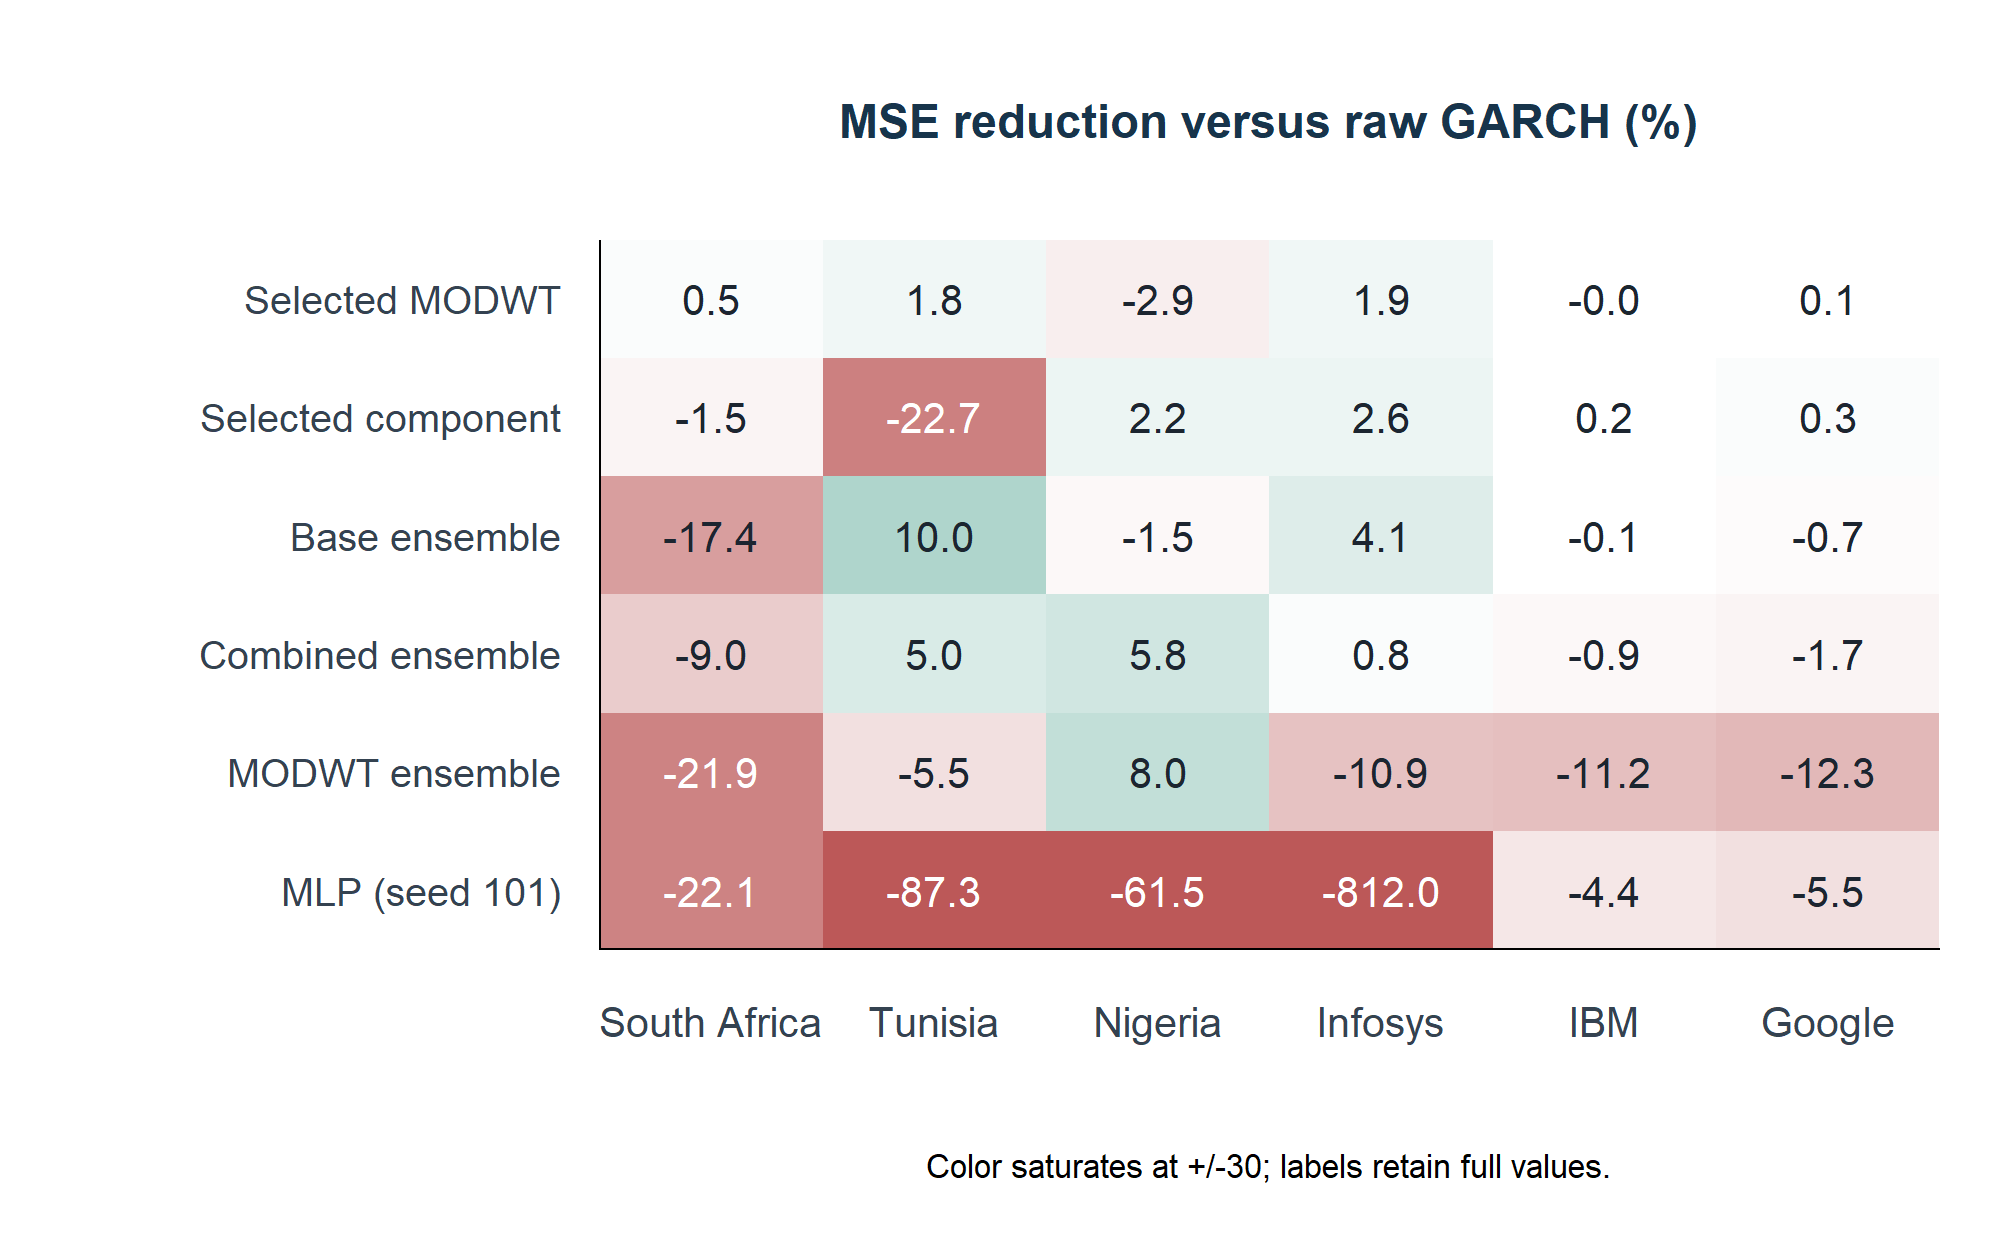
\includegraphics[width=\columnwidth]{figures/historical_extension_gains.png}
\caption{MSE gain vs.\ raw GARCH (\%) on the 2012--2014 test, pairwise matched dates. Green is better, red is worse.}
\label{fig:gain}
\end{figure}

Figure~\ref{fig:gain} gives the gains of the extensions on the test. The validation-selected MODWT model (Gaussian, structural or Student-t, as chosen per series) gains between $-2.9\%$ and $+1.9\%$, so the E2 order rule did not change much. The selected component model is good on Nigeria ($+2.2\%$) and Infosys ($+2.6\%$) but bad on Tunisia ($-22.7\%$), where the one huge spike in early 2013 hurts a model that works on the target directly. Most of the 24 component variants were much worse than raw GARCH: out of 144 series--variant pairs only 9 beat it and 123 were more than 10\% worse. For example on South Africa the db4 and db6 all-ARMA versions had more than 100\% higher MSE. Smoothing the target with a two-sided filter and then forecasting at the edge does not work well.

The ensembles give mixed results. The base ensemble gains 10.0\% on Tunisia and 4.1\% on Infosys but loses 17.4\% on South Africa. The combined ensemble gains on Tunisia, Nigeria and Infosys. The MODWT ensemble is worse on five of six series (about $-11\%$ on the three stocks) because it contains component models that are weak.

The MLP is the weakest model. With seed 101 it is worse than raw GARCH on every series, from $-4.4\%$ on IBM to $-812\%$ on Infosys, where one bad seed gave a few huge forecasts. The three seeds also disagree a lot: on Infosys the RMSE is 33.27, 24.09 and 33.27 for seeds 101, 202 and 303, against 23.17 for raw GARCH on the same 199 dates. With only about 1,000 noisy training points and 7 inputs, the network can not learn anything that GARCH does not already capture, and it is unstable.

\subsection{Sensitivity (E6)}

Changing the window(40 or 60 days), using BIC, or raising the order cap to 5 moved the test MSE of the core pipelines by less than about 2.6\% in all cases. The window length changed the results a lot. A longer window of 1,536 lowered the MSE of raw GARCH by 7.9\% on Tunisia and 7.2\% on Nigeria, while a shorter window of 768 increased it by 14.4\% on Tunisia. For the stocks the window effect was below 2\%. So for these markets, more history gives more stable GARCH parameters, and the choice of window is more important than the choice of wavelet.

\subsection{Later stock period, 2015--2025 (E7)}

\begin{table}[t]
\caption{MSE gain vs.\ raw GARCH (\%), frozen models. Test = 2012--2014, Later = 2015--2025. Pairwise matched dates.}
\label{tab:later}
\centering\small
\setlength{\tabcolsep}{3pt}
\begin{tabular}{lrrrrrr}
\toprule
 & \multicolumn{2}{c}{Infosys} & \multicolumn{2}{c}{IBM} & \multicolumn{2}{c}{Google}\\
Model & Test & Later & Test & Later & Test & Later\\
\midrule
DWT & 3.0 & 2.6 & $-1.4$ & 1.7 & $-0.1$ & $-5.5$\\
MODWT & 0.8 & 0.3 & 0.0 & 0.1 & 0.1 & $-0.3$\\
Ens.\ base & 4.1 & 1.4 & $-0.1$ & $-0.5$ & $-0.7$ & 1.4\\
Ens.\ comb. & 0.8 & 1.4 & $-0.9$ & $-0.8$ & $-1.7$ & 1.2\\
Ens.\ MODWT & $-10.9$ & $-6.6$ & $-11.2$ & $-10.3$ & $-12.3$ & $-7.4$\\
MLP & $-812$ & $-52.5$ & $-4.4$ & $-51.1$ & $-5.5$ & $-71.2$\\
\bottomrule
\end{tabular}
\end{table}

Table~\ref{tab:later} runs the same models on eleven more years of stock data. The results are the same. MODWT stays within 0.3\% of raw GARCH. DWT keeps its gain on Infosys (2.6\%), turns slightly positive on IBM, and is worse on Google. The MODWT ensemble and the MLP perform clearly worse. Small gains can flip sign between periods (for example the ensembles on Google).

%=====================================================================
\section{Conclusion}
\label{sec:conc}

We rebuilt the wavelet + ARMA--GARCH approach of \citet{ismail2016} from scratch and tested it  on six markets. Our observations are the following:
\begin{itemize}
\item The wavelet step does not improve predictions a lot. MODWT-GARCH performs almost the same as plain GARCH everywhere. DWT-GARCH helps on Nigeria and Infosys, and Tunisia (3--9\% lower MSE), but not on IBM, Google or South Africa. So we could not confirm the paper's result that the wavelet model is better on every market.
\item How the wavelet forecast is mapped back to the return variance matters a lot. For the paired DWT, conditioning on the already-observed first return of the pair is necessary; without it the variance forecast is far too high.
\item Returns do not follow a normal distribution, and Student-t or GED additions give small but consistent gains, the most improvement is seen on the fattest-tailed series (Tunisia).
\item A plain GARCH(1,1) is very hard to beat. Ensembles help only when all members perform better, and a small MLP performs worse and is unstable.
\item The rolling window length had a bigger effect than the wavelet choice on some markets.
\end{itemize}

\textbf{Limitations.} The difference in errors of all methods is very small. The obtained target is a noisy proxy for true volatility. We used only Haar wavelets for the core pipelines and first-level transforms. The 2015--2025 stock period is retrospective.


\section{Future Work}
Our next steps are:
\begin{itemize}
\item\textbf{Formal tests:} Model Confidence Set,Diebold-Mariano
\item \textbf{Using Asymmetric Models:} Frameworks like EGARCH or GJR-GARCH can be used to account for the leverage effect, where bad news increases volatility more than good news.
\item\textbf{Deeper Window:}We can experiment with deeper wavelet levels and other filters inside the return pipelines and weights can be learned on validation instead of equal weights.
\end{itemize}

\bibliography{refs}
\bibliographystyle{icml2018}

\end{document}
